\section{Green's Functions}

\subsection{Physical motivation: Static Forces on a String}
Consider a \underline{massive} static string with tension $T$ and linear mass density $\mu$, suspended between fixed ends ($L = 1$)
\begin{align} \label{eq:7.1}
    y(0) = y(1) = 0.
\end{align}
By resolving forces, we have the time independent form \cref{eq:3.3}
\begin{align*}
	T \dv[2]{y}{x} - \mu g = 0
\end{align*}
We will solve the inhomogeneous ODE 
\begin{align} \label{eq:7.2}
    - \dv[2]{y}{x} = f(x)
\end{align} with $f(x) = -\frac{\mu g}{T}$ subject to $\cref{eq:7.1}$.

\subsubsection{Direct integration}
This has been placed in Sturm-Liouville form.
We can integrate directly and find $\cref{eq:7.2}$ gives
\begin{align*}
	-y = -\frac{\mu g}{2T} x^2 + k_1 x + k_2
\end{align*}
Imposing boundary conditions \cref{eq:7.1},
\begin{align} \label{eq:7.3}
	y(x) = \qty(-\frac{\mu g}{T}) \cdot \frac{1}{2}x(1-x)
\end{align}

\subsubsection{Superposition of point masses}
Consider alternatively a solution obtained by solving the equation for a single point mass $\delta m = \mu \delta x$ suspended at $x = \xi_i$ on an very light string.
We can then superimpose the solutions for each point mass to find the overall solution.
For a single point mass, the solution is given by two straight lines from $(0,0)$ and $(1,0)$ to the point mass $(\xi_i, y_i(\xi_i))$.
The angles of these straight lines from the horizontal are given by $\theta_1, \theta_2$.
\begin{figure}[h] 
    \centering 
    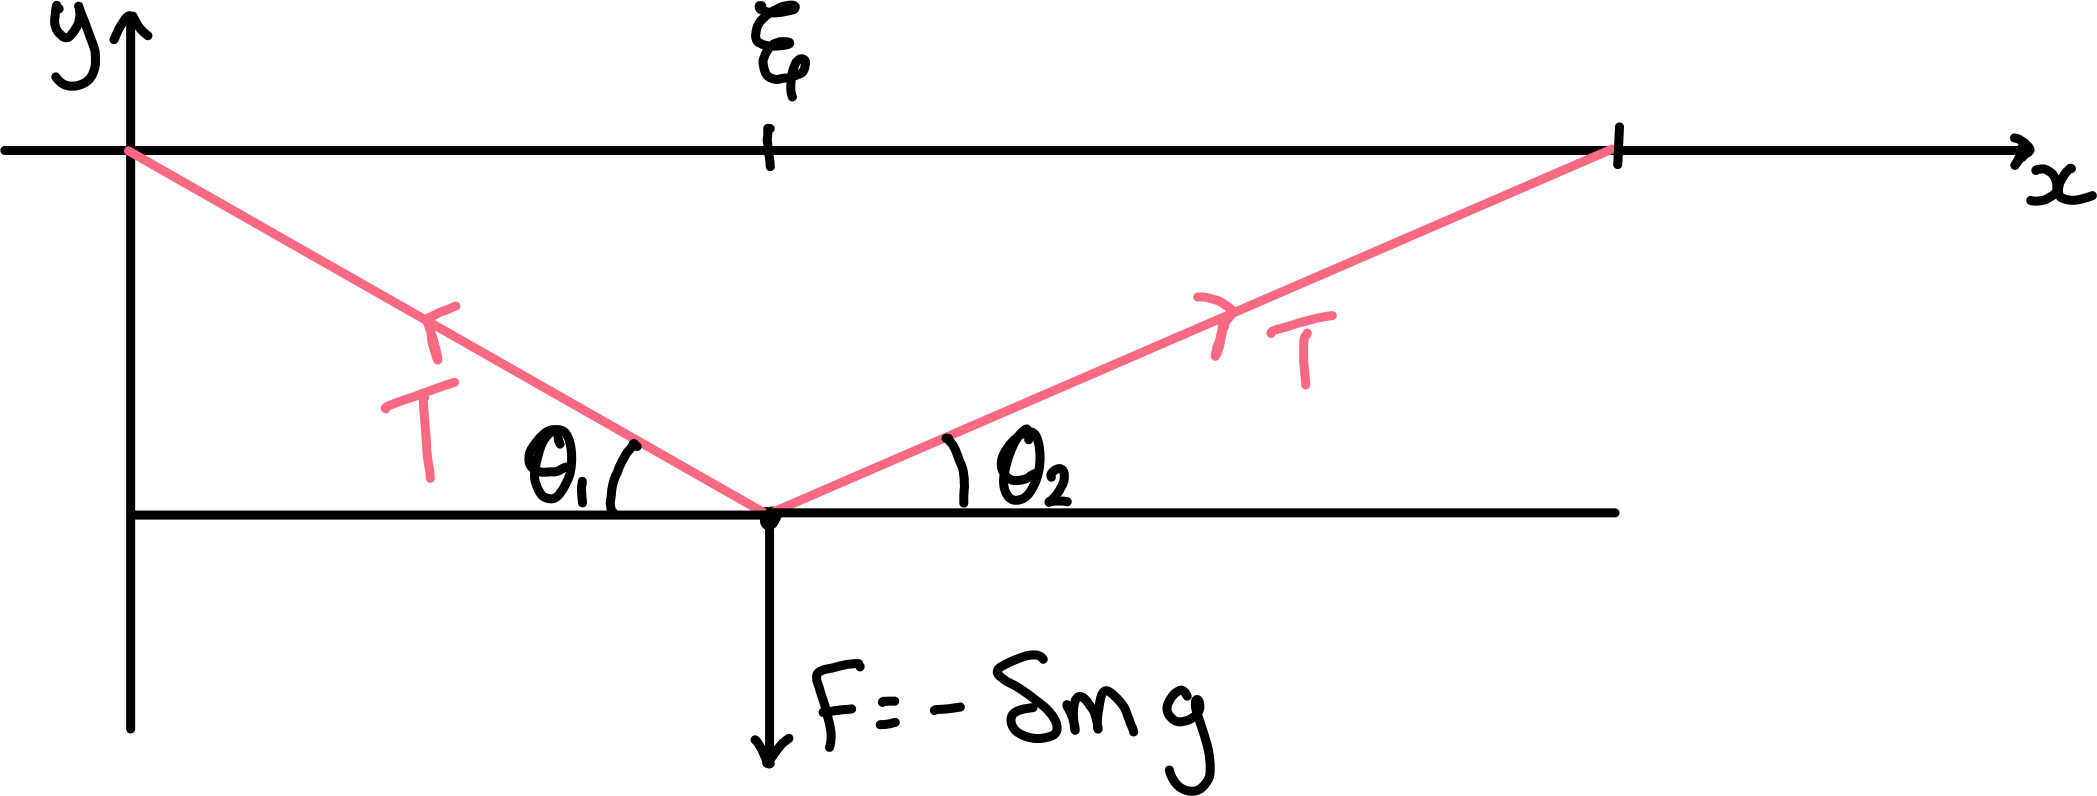
\includegraphics[height=5cm]{07-stringdiagram} 
\end{figure}
Resolving in the $y$ direction to find $y_i(\xi_i)$,
\begin{align*}
	0 & = T (\sin \theta_1 + \sin \theta_2) - \delta m g \\
	& = T\qty(\frac{-y_i}{\xi_i} + \frac{-y_i}{1-\xi_i}) - \delta m g \\
	\therefore -T\qty(y_i(1-\xi_i) + y_i \xi_i) & = \delta m g \xi_i(1-\xi_i) \\
	\therefore y_i(\xi_i) & = \frac{-\delta m g}{T} \xi_i (1-\xi_i)
\end{align*}
So the solution is
\begin{align*}
	y_i(x) = \frac{-\delta m g}{T} \begin{cases}
		x(1-\xi_i)    & x < \xi_i \\
		\xi_i (1 - x) & x > \xi_i
	\end{cases}
\end{align*}
which is the generalised sawtooth.
This can alternatively be written
\begin{align*}
	y_i(x) = f_i(\xi) G(x,\xi)
\end{align*}
where $f_i$ is a source term, and $G(x,\xi)$ is the Green's function, the solution for a unit point source.
Since the differentialan analogous result to Parseval’s theorem equation is linear, we can sum the solutions for $N$ point masses, giving
\begin{align*}
	y(x) = \sum_{i=1}^N f_i(\xi) G(x, \xi_i)
\end{align*}
Taking a \underline{continuum limit},
\begin{align*}
	f_i(\xi) = \frac{-\delta m g}{T} = \frac{-\mu \delta x g}{T} \equiv f(x) \dd{x} \implies f(x) = \frac{-\mu g}{T}
\end{align*}
which gives ($x \mapsto \xi$)
\addtocounter{equation}{1}
\begin{align} \label{eq:7.5}
	y(x) = \int_0^1 f(\xi) G(x,\xi) \dd{\xi}
\end{align}
where we are integrating over all source positions.
Substituting the Green's function,
\begin{align*}
	y(x) & = \qty(\frac{-\mu g}{T}) \qty[ \underbracket{\int_0^x \xi(1-x) \dd{\xi}}_{x > \xi} + \underbracket{\int_x^1 x(1-\xi) \dd{\xi}}_{x < \xi}] \\
    &= \qty(\frac{-\mu g}{T}) \qty{ \qty[\frac{\xi^2}{2}(1-x)]_0^x + \qty[x \qty(\xi - \frac{\xi^2}{2})]_x^1 } \\
    &= \qty(\frac{-\mu g}{T}) \qty(\frac{x^2}{2}(1-x) - 0 + \frac{x}{2} - x\qty(x-\frac{x^2}{2}))  \\
    &= \qty(\frac{-\mu g}{T}) \cdot \frac{1}{2}x(1-x)
\end{align*}
So we have found the correct solution in two ways; once by direct integration, and once by superimposing point solutions.
In general, direct integration is not trivial, and Green's functions are useful in this case.

\subsection{Definition of Green's function}
We wish to solve the inhomogeneous ODE \cref{eq:2.21}
\begin{align} \label{eq:7.6}
	\mathcal L y \equiv \alpha(x) y'' + \beta(x) y' + \gamma(x) y = f(x)
\end{align}
on $a \leq x \leq b$, where $\alpha \neq 0$ and $\alpha, \beta, \gamma$ are continuous and bounded, taking homogeneous boundary conditions $y(a) = y(b) = 0$. \\
The Green's function for $\mathcal L$ in this case is defined to be the solution for a unit point source at $x = \xi$.
That is, $G(x,\xi)$ is the function that satisfies the boundary conditions and
\begin{align} \label{eq:7.7}
	\mathcal L G(x,\xi) = \delta(x-\xi)
\end{align}
so $G(a,\xi) = G(b,\xi) = 0$.
Then, by linearity, the general solution is given by
\begin{align} \label{eq:7.8}
	y(x) = \int_a^b f(\xi) G(x,\xi) \dd{\xi}
\end{align}
where $y(x)$ satisfies the homogeneous boundary conditions.
We can verify this by checking
\begin{align*}
	\mathcal L y = \int_a^b \mathcal L_{(x)} G(x,\xi) f(\xi) \dd{\xi} = \int_a^b \delta(x-\xi) f(\xi) \dd{\xi} = f(x)
\end{align*}
So the solution is given by the inverse operator
\begin{align*}
	y = \mathcal L^{-1} f;\quad \mathcal L^{-1} = \int_a^b \dd{\xi} G(x,\xi)
\end{align*}

\subsection{Defining properties (summary)}
The Green's function spits into two parts;
\begin{align} \label{eq:7.9}
	G(x,\xi) = \begin{cases}
		G_1(x,\xi) & a \leq x < \xi \\
		G_2(x,\xi) & \xi < x \leq b
	\end{cases}
\end{align}
\begin{enumerate}
    \item \underline{Hom solns} $G$ solves homogenous equation $\forall \; x \neq \xi$ so 
    \begin{align} \label{eq:7.10}
        \mathcal L G_1 = \mathcal L G_2 = 0
    \end{align} 
    \item \underline{Hom b.c.s} $G$ satisfies the homogeneous boundary conditions, so 
    \begin{align} \label{eq:7.11}
        G_1(a, \xi) = 0,\quad G_2(b, \xi) = 0
    \end{align} 
    \item \underline{Continuity condition} $G$ must be continuous at $x = \xi$, hence
    \begin{align} \label{eq:7.12}
        G_1(\xi, \xi) = G_2(\xi, \xi)
    \end{align} 
    \item \underline{Jump condition} There is a jump condition; the derivative of $G$ is discontinuous at $x = \xi$.
    This satisfies
    \begin{align} \label{eq:7.13}
        [G']_{\xi_-}^{\xi_+} = \eval{\dv{G_2}{x}}_{x = \xi_+} - \eval{\dv{G_1}{x}}_{x = \xi_-} = \frac{1}{\alpha(\xi)}
    \end{align}
    where $\alpha(x)$ is defined in \cref{eq:7.6}.
\end{enumerate} 

\subsection{Explicit form for Green's functions}
We want to solve
\begin{align*}
	\mathcal L G(x,\xi) = \delta(x-\xi)
\end{align*}
on $a \leq x \leq b$, subject to homogeneous boundary conditions $G(a,\xi) = G(b,\xi) = 0$.
The functions $G_1, G_2$ satisfy the homogeneous equation, so $\mathcal L G_i(x,\xi) = 0$.
Suppose there exist two independent homogeneous solutions $y_1(x), y_2(x)$ to $\mathcal L y = 0$.
Then, $G_1 = A y_1 + B y_2$, such that $A y_1(a) + B y_2(a) = 0$, which gives a constraint between $A$ and $B$.
This defines a complementary function $y_-(x)$ such that $y_-(a) = 0$.
The general homogeneous solution with $G_1(a) = 0$ is
\begin{align*}
	G_1 = C y_-
\end{align*}
$C$ will be found later.
Similarly we can define $y_+$ as a linear combination of $y_1, y_2$ such that $y_+(b) = 0$.
\begin{align*}
	G_2 = D y_+
\end{align*}
We require $G_1(\xi, \xi) = G_2(\xi, \xi)$ for continuity, hence
\begin{align*}
	C y_-(\xi) = D y_+(\xi)
\end{align*}
Since $[G']_{\xi_-}^{\xi^+} = \frac{1}{\alpha(\xi)}$, we have
\begin{align*}
	Dy'_+(\xi) - C Y_-'(\xi) = \frac{1}{\alpha(\xi)}
\end{align*}
We can solve these equations for $C, D$ simultaneously to find
\begin{align*}
	C(\xi) = \frac{y_+(\xi)}{\alpha(\xi)W(\xi)};\quad D(\xi) = \frac{y_-(\xi)}{\alpha(\xi)W(\xi)}
\end{align*}
where $W(\xi)$ is the Wro\'nskian
\begin{align*}
	W(\xi) = y_-(\xi) y_+'(\xi) - y_+(\xi) y_-'(\xi)
\end{align*}
which is nonzero if $y_-, y_+$ are linearly independent.
Hence,
\begin{align*}
	G(x,\xi) = \begin{cases}
		\frac{y_-(x) y_+(\xi)}{\alpha(\xi)W(\xi)} & a \leq x \leq \xi \\
		\frac{y_-(\xi) y_+(x)}{\alpha(\xi)W(\xi)} & \xi \leq x \leq b
	\end{cases}
\end{align*}

\subsection{Solving boundary value problems}
We know that the solution of $\mathcal L y = f$ is
\begin{align*}
	y(x) = \int_a^b G(x,\xi) f(\xi) \dd{\xi}
\end{align*}
We can split this into two intervals given that $G = G_1$ for $\xi > x$ and $G = G_2$ for $\xi < x$.
\begin{align*}
	y(x) & = \int_a^x G_2(x,\xi) f(\xi) \dd{\xi} + \int_x^b G_1(x,\xi) f(\xi) \dd{\xi} \\
    & = y_+(x) \int_a^x \frac{y_-(\xi) f(\xi)}{\alpha(\xi)W(\xi)} \dd{\xi} + y_-(x) \int_a^x \frac{y_+(\xi) f(\xi)}{\alpha(\xi)W(\xi)} \dd{\xi}
\end{align*}
Note that if $\mathcal L$ is in Sturm-Liouville form, so $\beta = \alpha'$, then the denominator $\alpha(\xi)W(\xi)$ is a constant.
Further, $G$ is symmetric; $G(x,\xi) = G(\xi,x)$.
Often, by convention, we take $\alpha = 1$ (however Sturm-Liouville form typically takes $\alpha < 0$).
\begin{example}
	Consider $y'' - y = f(x)$ with $y(0) = y(1) = 0$.
	Homogeneous solutions are $y_1 = e^x$, $y_2 = e^{-x}$.
	Imposing boundary conditions,
	\begin{align*}
		G = \begin{cases}
			C \sinh x    & 0 \leq x < \xi \\
			D \sinh(1-x) & \xi < x \leq b
		\end{cases}
	\end{align*}
	Continuity at $x = \xi$ implies
	\begin{align*}
		C \sinh \xi = D \sinh (1 - \xi) \implies C = D \frac{\sinh (1-\xi)}{\sinh \xi}
	\end{align*}
	The jump condition is
	\begin{align*}
		-D \cosh(1-\xi) - C \cosh \xi = 1
	\end{align*}
	Hence,
	\begin{align*}
		-D\qty[\cosh(1-\xi)\sinh \xi + \sinh(1-\xi)\cosh \xi] & = \sinh \xi  \\
		-D\qty[\sinh((1-\xi) + \xi)] &= \sinh \xi \\
		-D\sinh 1 &= \sinh \xi \\
		D &= \frac{\sinh \xi}{\sinh 1} \\
		\therefore C &= \frac{-\sinh(1-\xi)}{\sinh 1}
	\end{align*}
	Therefore,
	\begin{align*}
		y(x) = \frac{-\sinh(1-x)}{\sinh 1} \int_0^x \sinh \xi f(\xi) \dd{\xi} - \frac{\sinh x}{\sinh 1} \int_x^1 \sinh (1-\xi) f(\xi) \dd{\xi}
	\end{align*}
\end{example}
\noindent Suppose we have inhomogeneous boundary conditions.
In this case, we want to find a homogeneous solution $y_p$ that solves the inhomogeneous boundary conditions.
That is, $\mathcal L y_p = 0$ but $y_p(a), y_p(b)$ are as required for the boundary conditions.
Then, by subtracting this solution from the original equation, we can solve using a homogeneous set of boundary conditions.
For instance, in the above example, suppose $y(0) = 0, y(1) = 1$.
We can find a solution $y_p = \frac{\sinh x}{\sinh 1}$ which has the inhomogeneous boundary conditions but solves the homogeneous problem.

\subsection{Higher-order ODEs}
Suppose $\mathcal L y = f(x)$ where $\mathcal L$ is an $n$th order linear differential operator, and $\alpha(x)$ is the coefficient for the highest degree derivative.
Suppose that homogeneous boundary conditions are satisfied.
Then we can define the Green's function in this case to be the function that solves
\begin{align*}
	\mathcal L G(x,\xi) = \delta(x-\xi)
\end{align*}
which has the properties:
\begin{enumerate}
	\item $G_1, G_2$ are homogeneous solutions satisfying the homogeneous boundary conditions;
	\item $G_1^{(k)}(\xi) = G_2^{(k)}(\xi)$ for $k \in \qty{0, \dots, n-2}$;
	\item $G_2^{(n-1)}(\xi^+) - G_1^{(n-1)}(\xi^-) = \frac{1}{\alpha(\xi)}$.
\end{enumerate}

\subsection{Eigenfunction expansions of Green's functions}
Suppose $\mathcal L$ is in Sturm-Liouville form with eigenfunctions $y_n(x)$ and eigenvalues $\lambda_n$.
We seek $G(x,\xi) = \sum_{n=1}^\infty A_n y_n(x)$ satisfying $\mathcal L G = \delta(x-\xi)$.
\begin{align*}
	\mathcal L G &= \sum_n A_n \mathcal L y_n \\
	&= \sum_n A_n \lambda_n w(x) y_n(x)
\end{align*}
The $\delta$ function has expansion
\begin{align*}
	\delta(x-\xi) = w(x) \sum_n \frac{y_n(\xi) y_n(x)}{N_n};\quad N_n = \int w y_n^2 \dd{x}
\end{align*}
Hence,
\begin{align*}
	A_n(\xi) = \frac{y_n(\xi)}{\lambda_n N_n}
\end{align*}
Thus,
\begin{align*}
	G(x,\xi) = \sum_{n=1}^\infty \frac{y_n(\xi) y_n(x)}{\lambda_n \int w y_n^2 \dd{x}} = \sum_{n=1}^\infty \frac{Y_n(\xi) Y_N(x)}{\lambda_n}
\end{align*}
which was already obtained earlier in the course when studying Sturm-Liouville theory.

\subsection{Constructing Green's function for an initial value problem}
Suppose we want to solve $\mathcal L y = f(t)$ for $t \geq a$ with $y(a) = y'(a) = 0$, using $G(t, \tau)$ satisfying $\mathcal L g = \delta(t - \tau)$.
For $t < \tau$, we have
\begin{align*}
	G_1 = A y_1(t) + B y_2(t);\quad A y_1(a) + B y_2(a) = 0;\quad A y_1'(a) + B y_2'(a) = 0
\end{align*}
If $A \neq B \neq 0$, then we can solve this by dividing out $A, B$ and find $y_1 y_2' - y_2 y_1' = 0$.
Since the Wro\'nskian at $a$ cannot be zero, $A = B = 0$.
So $G_1(t,\tau) \equiv 0$ for $a \leq t < \tau$, so there is no change until the `impulse' at $t = \tau$.

For $t > \tau$, by continuity we must have $G_2(\tau, \tau) = 0$.
So we choose a complementary function $G_2 = D y_+(t)$ with $y_+(t) = A y_1(t) + B y_2(t)$, and $y_+(\tau) = 0$.
The discontinuity in the derivative implies that
\begin{align*}
	G_2'(\tau, \tau) = Dy_+'(\tau) = \frac{1}{\alpha(\tau)}
\end{align*}
Hence,
\begin{align*}
	A y_1'(\tau) + B y_2'(\tau) = \frac{1}{\alpha(\tau)} \implies D(\tau) = \frac{1}{\alpha(\tau) y_+'(\tau)}
\end{align*}
Hence we have a non-trivial solution
\begin{align*}
	G(t, \tau) = \begin{cases}
		0 & t < \tau \\
		\frac{y_+(t)}{\alpha(\tau) y_+'(\tau)} & t > \tau
	\end{cases}
\end{align*}
The initial value problem has solution
\begin{align*}
	y(t) = \int_a^t G_2(t, \tau) f(\tau) \dd{\tau} = \int_a^t \frac{y_+(t) f(\tau)}{y_+'(\tau)} \dd{\tau}
\end{align*}
Causality is `built in' to this solution.
Only forces which occur before $t$ may have an impact on $y(t)$.
\begin{example}
	Let us solve $y''-y = f(t)$ with $y(0) = y'(0) = 0$.
	The homogeneous solution and initial conditions are
	\begin{align*}
		t < \tau \implies G_1 \equiv 0
	\end{align*}
	and
	\begin{align*}
		t > \tau \implies G_2 = A e^t + Be^{-t} = D \sinh (t - \tau)
	\end{align*}
	Now,
	\begin{align*}
		[G']_{\tau_-}^{\tau_+} = \frac{1}{\alpha(\tau)} = 1 \implies G'(\tau, \tau) = D \cosh 0 = D = 1
	\end{align*}
	Hence, the solution is
	\begin{align*}
		y(t) = \int_0^t f(\tau) \sinh (t - \tau) \dd{\tau}
	\end{align*}
\end{example}